\section{Nebulas Rank}
\label{sec:rank}

\subsection{价值尺度总体设计} \label{subsec:value}
当前区块链技术和生态已具有相当规模,但是人们对其认识还处于扁平化阶段,尚不存在一个合理的方式去评估链上实体(例如用户地址)的价值。因此,我们试图在区块链世界提出⼀个普适的价值尺度,通过对链上行为的挖掘利用,将每个实体(用户地址)的重要程度量化为\textbf{Nebulas Rank}的指标形式。\textbf{Nebulas Rank}旨在实现双重目标:
\begin{itemize}
	\item 作为原生的价值尺度,\textbf{Nebulas Rank}可以成为诸多基础场景的核心算法,如共识算法(见\refsec{sec:pod})、开发者激励(见\refsec{sec:dip})和区块链搜索引擎(见\refsec{sec:search}),等等;
	\item \textbf{Nebulas Rank}可以启发人们对区块链的生态现状定义更多样化的价值尺度,同时产生更深层次、差异化和结构化的认识,进而在商业决策和研究活动中有明确的方向;
\end{itemize}
基于上述目标,我们为\textbf{Nebulas Rank}定义了三重价值尺度:
\begin{itemize}
	\item 流动性,即交易的频次和规模,是\textbf{Nebulas Rank}的第⼀个考量维度。本质上来看,⾦融是通过资本流动推动社会资源的有效配置、推动经济发展的社会活动。区块链构建了⼀个价值⽹络,更多的交易数量、更⼤的交易规模产⽣更⾼的流动性,更⾼的流动性⼜进⼀步提升了交易数量、交易规模,从⽽进⼀步强化了它们的价值,形成了⼀个完整的正向反馈机制。 
	\item 传播性,即资产流动的⼴度和深度,是\textbf{Nebulas Rank}的第⼆个考量维度。在社交网络中的传播性,即信息的传播速度、⼴度和深度,是⽹络质量和⽤户增长的关键指标。我们在区块链世界将会看到同样的模式,强⼤传播性意味着资产流动的⼴度和深度,会提⾼区块链世界的资产质量,提升资产规模。
	\item 互操作性是\textbf{Nebulas Rank}的第三个考量维度。在互联⽹的早期,我们只有简单的⽹站,孤⽴的信息。现在,⽹络上的各种平台信息开始相互调⽤,数据孤岛逐渐被打破。这⼀趋势可以被理解为识别更⾼维度信息的过程。我们认为区块链世界也会遵循同样的发展规律,但其过程速度会更快。⽤户的资产、智能合约和DApp之间的信息会越来越丰富,⾼维信息间的互操作会越来越频繁,因此更好的互操作性将会变得越来越重要。 
\end{itemize}

我们选择使用链上的交易记录作为\textbf{Nebulas Rank}算法的数据来源。因为相比于现实世界,区块链世界的『行踪』更为清晰和可信:链上的交易数据忠实地记录了用户之间的每笔转账、以及每次对『智能合约』的调用情况。然而根据交易数据设计算法并非易事。因为相比于现实世界,区块链世界的交易具有天然的匿名性,同时数据量规模更为庞大。因此我们试图为\textbf{Nebulas Rank}刻画如下的性质:
\begin{itemize}
	\item 可信。实体如果要提高自己的价值,必须付出一定的成本,这样可以确保算法的结果能够甄选出真正具有较高价值的用户。一方面,在共识算法和开发者激励等场景下,可信的结果鼓励用户诚实地贡献以实现正向反馈,另一方面,可信的结果提供了有意义的用户分层结果,能提供更好的决策基础。
	\item 可计算。作为基础算法,\textbf{Nebulas Rank}的结果以每个用户的链上字段的形式呈现,因此其实现需要较低的计算复杂度;
	\item 可复现。由于共识算法和开发者激励等场景的需要,\textbf{Nebulas Rank}需要保证在所有客户端的计算结果完全一致。
\end{itemize}

接下来我们设计\textbf{Nebulas Rank}的基本框架。首先,我们用图的形式表现交易记录。在交易图的基本定义中,每个节点代表一个实体,每条边代表实体之间的转账行为\cite{Tschorsch2015}。交易图表现了转账行为导致资产流动的性质,有助于表示上述价值尺度中流动性和传播性的概念。同时,图的形式也能方便刻画合约之间的互操作性。得到图之后便可以用复杂网络的中心性测度来对重要网络节点进行排序,对\textbf{Nebulas Rank}的情景,我们采用LeaderRank\cite{Chen2013}\cite{Li2014},并取得比PageRank和NEM\cite{nem}的NCDAwareRank更好的排序效果。

\subsection{交易图} \label{subsec:txg}
本小节介绍如何从交易数据构造交易图。

首先,取近期$T$个区块内个人用户对个人用户的有效转账记录,记为$T_{xs}$:
\begin{align}
T_{xs} = \{(s,t,\tau, a)| \tau = \#CurrentBlock-T \dots \#CurrentBlock \land a > 0 \}
\end{align}
,$s$、$t$和$a$分别是转出地址、转入地址和转账金额。

然后基于$T_{xs}$,构造有向加权简单图$G=(V, E, W)$,其中,节点集合、边集合和边权分别表示为$V$, $E$和$W$。另外,记$N = |V|$,$M = |E|$。 简便起见,所有节点都以一个$1$到$N$之间的整数代表。

每个节点都代表一个账户的地址,每条边代表两个用户之间的转账强度。规定所有边有向,并按如下公式合并对应交易的最高$K$个金额作为权值$w_e$:
\begin{align}\label{formula:edgeweight}
w_e = \sum_{i=1}^K a_i, s.t. a_i \in \{a|(s,t,\tau,a) \in T_{xs} \} \land a_1 \geq a_2 \dots
\end{align}

接着,对每个节点,根据其在过去$T$个区块的转入转出行为,计算它的『币龄』,记作$C_v$,并且根据$C_v$对邻接边的权值进行衰减。

最后,取整个交易图的最大弱连通分支,将分支之外的节点删除。

上述构造交易图的方式有助于实现\refsec{subsec:value}定义的『可信』性质:
\begin{itemize}
	\item 由于设置了$T$个区块的滑动时间窗,攻击者无法在短期内迅速提高自己的排名;
	\item 因为边权由最高的几次交易金额决定,在一个环状拓扑内的多次转账不能无限提高各边权值;
	\item 为了获得更高『币龄』,用户需要让资金在自己的账户内『停留』一段时间,进而拖慢攻击者伪造交易的速度;
\end{itemize}

本小节的剩余内容展示交易数据和交易图的部分结果。我们收集了\#3629091(约2017年5月1日)到\#3800775(2017年5月31日)共$171,684$个区块交易数据:
\begin{itemize}
	\item 个人用户之间的有效转账交易共有$2,567,832$条,参与交易的地址有$712,354$个,每次交易的平均金额为$\Xi 196.81$,每次交易的金额分布如\ref{fig:txad}所示,大多数交易的金额都在$\Xi 100$以下。每对地址的交易次数分布如\reffig{fig:txnd}所示,有$91\%$的双方只进行了一或两次交易,因此$K$取$2$是合适的。
	\item 交易图有$453,285$个节点,$970,577$条边。有$1,169$个弱分支,其中最大弱分支有$449,746$个节点,占全体节点的$99.2\%$,次大弱分支有$133$个节点,仅占全体节点的$0.03\%$,因此取最大弱联通分支有助于去除少数噪声节点。
	\item 合并交易、取最大弱连通分支后,可视化结果如\reffig{fig:wgc}所示。平均每个节点有$4.3$个邻居,节点邻居数的分布如\reffig{fig:nnd}所示。平均度(邻接边权值和)为$2070$。度(邻接边权值和)分布如\reffig{fig:nwd}所示,出度与入度的相关系数为$0.645$($p$-value$<0.001$),二者关系如\reffig{fig:nio}所示。
\end{itemize}

\begin{figure}
	\centering
	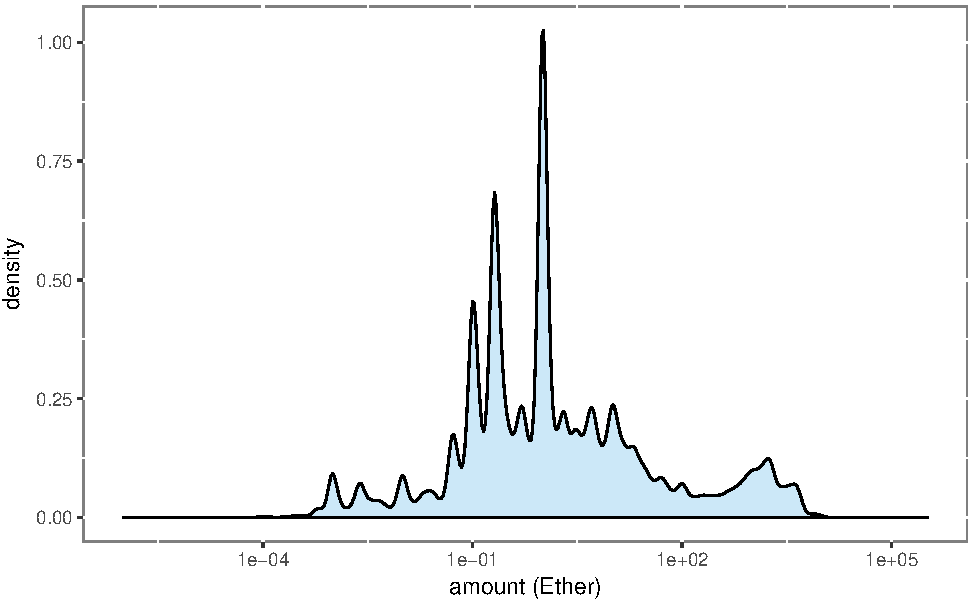
\includegraphics[width=0.85\textwidth]{figs/txad.pdf}
	\caption{单次交易金额分布 \\ \small{(横坐标为对数形式)}}\label{fig:txad}
\end{figure}

\begin{figure}
\centering
	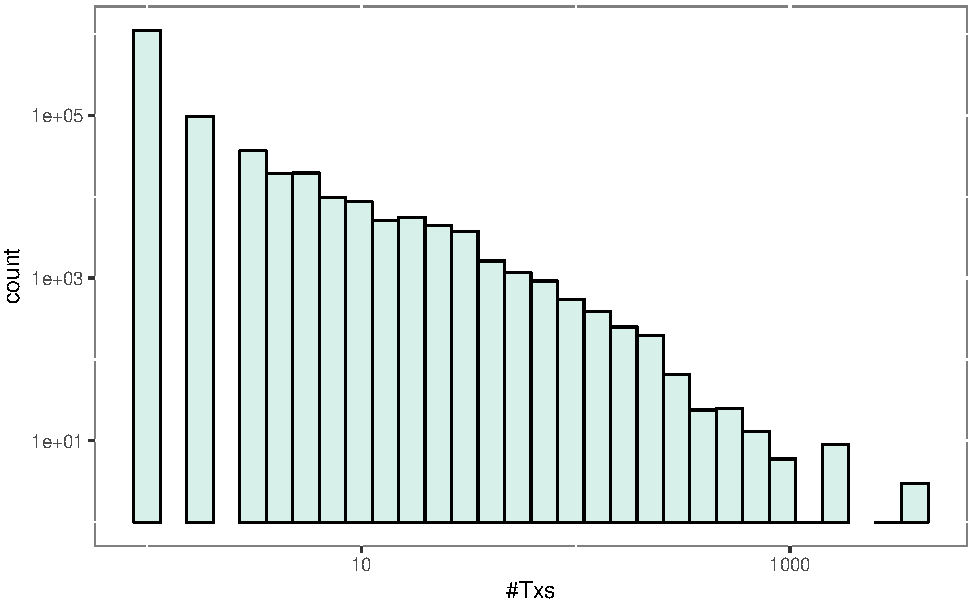
\includegraphics[width=0.85\textwidth]{figs/txnd.pdf}
	\caption{每对用户交易次数统计 \\ \small{(横纵坐标均为对数形式)}}\label{fig:txnd}
\end{figure}

\begin{figure}
	\centering
	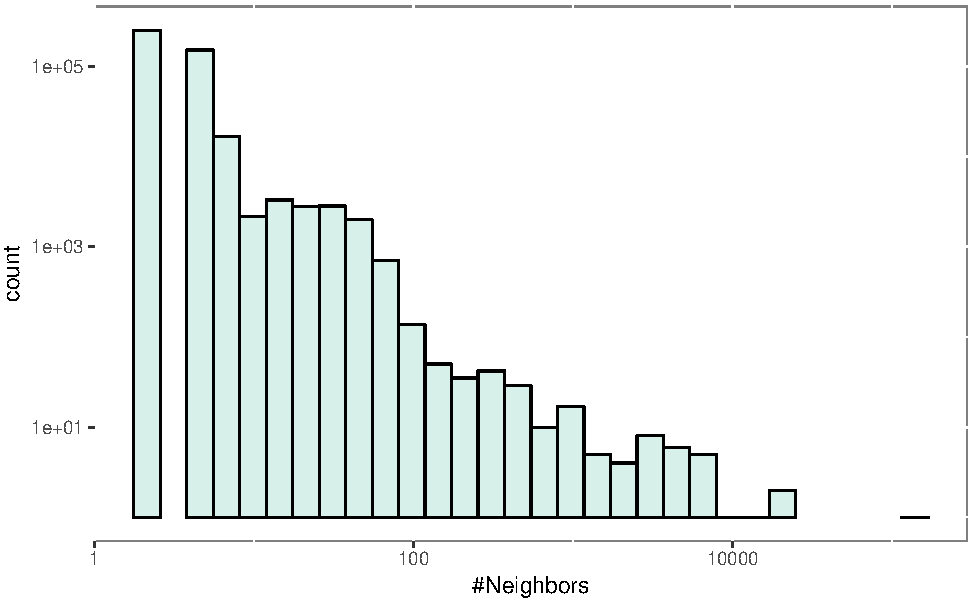
\includegraphics[width=0.85\textwidth]{figs/nnd.pdf}
	\caption{节点邻居数分布 \\ \small{(横纵坐标均为对数形式)}}\label{fig:nnd}
\end{figure}

\begin{figure}
	\centering
	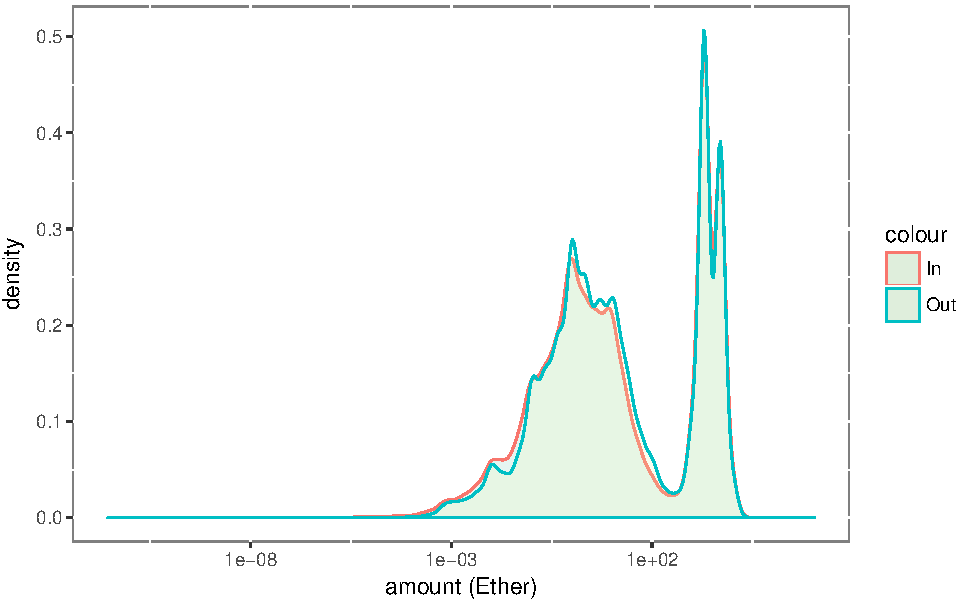
\includegraphics[width=0.85\textwidth]{figs/nwd.pdf}
	\caption{节点加权度分布 \\ \small{(横坐标为对数形式)} } \label{fig:nwd}
\end{figure}

\begin{figure}
	\centering
	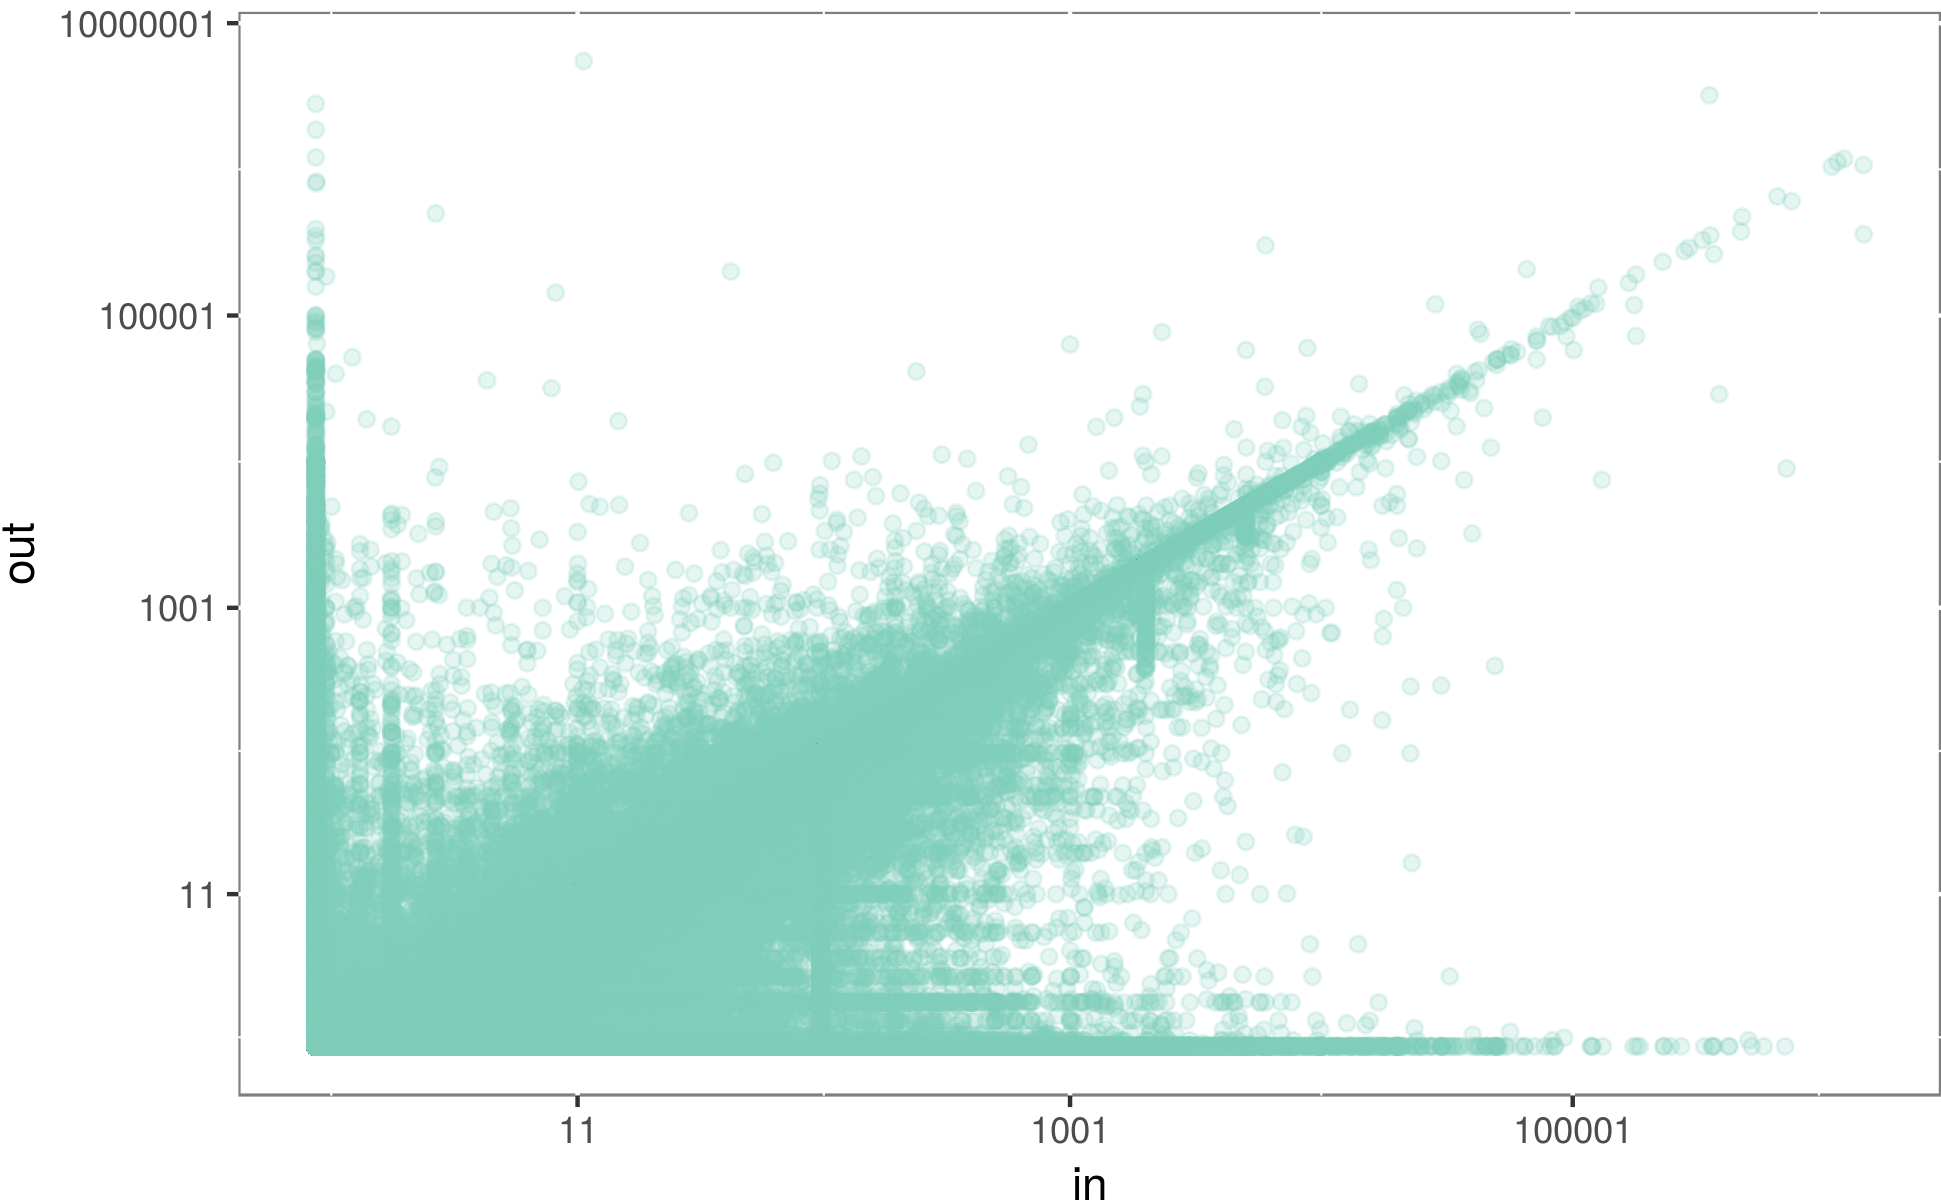
\includegraphics[width=0.85\textwidth]{figs/nio.png}
	\caption{节点加权出入度关系}\label{fig:nio}
\end{figure}

\begin{figure}
	\centering
	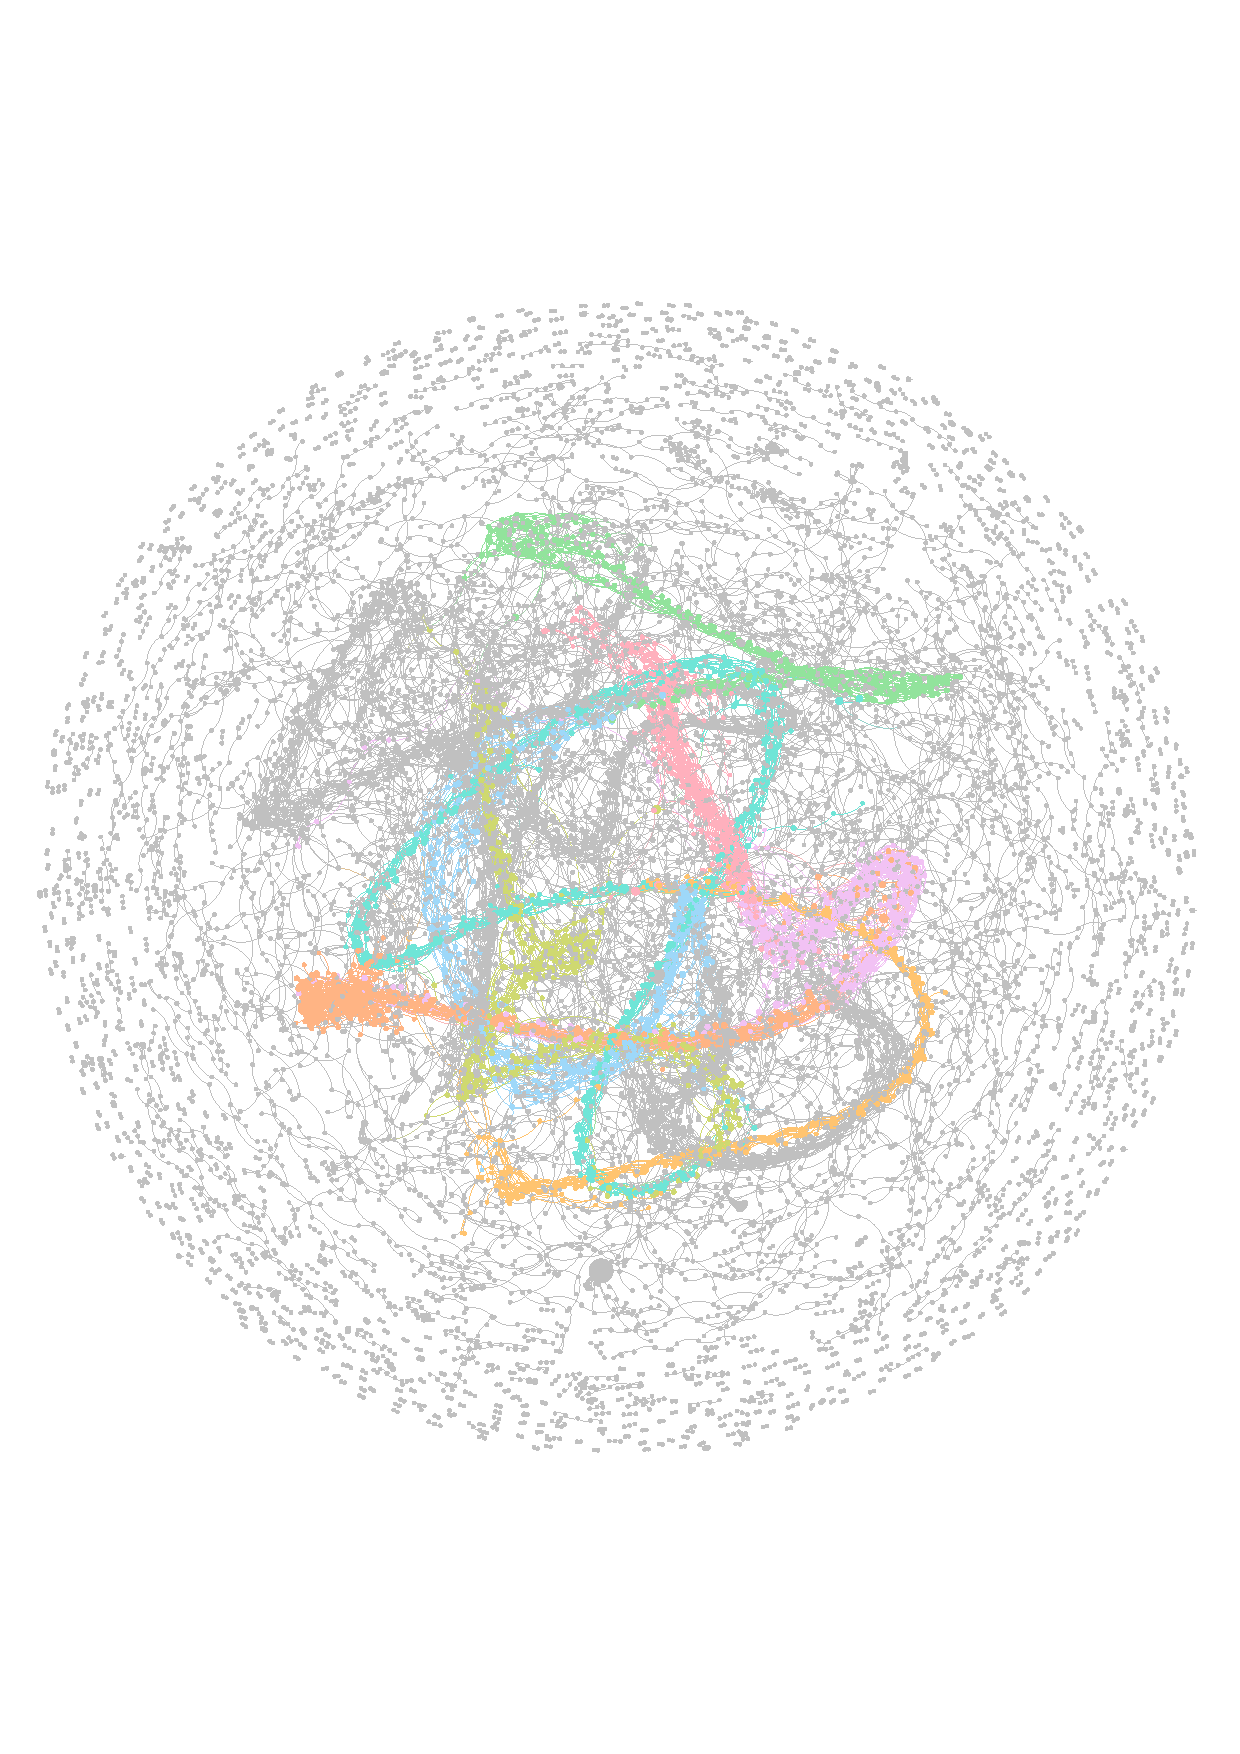
\includegraphics[width=0.85\textwidth]{figs/wgc.pdf}
	\caption{交易图可视化结果}\label{fig:wgc}
\end{figure}

\subsection{排序算法} \label{subsec:leaderrank}
本小节介绍如何在构造的图中进行节点重要性排序。

我们采用LeaderRank\cite{Chen2013}\cite{Li2014}作为核心算法。首先在交易图中添加Ground节点,记为$\mathcal{G}$,编号$N+1$。然后我们建立Ground节点和其他每个节点的双向链接,并按照接下来的方式赋予链接权值:
\begin{align}\label{formula:weight1}
	\forall v \in V, w_{(v, \mathcal{G})} = \alpha A_v
\end{align}
\begin{align}\label{formula:weight2}
\forall v \in V,  w_{(\mathcal{G}, v)} = \beta B_v
\end{align}
其中:
\begin{align}
	\forall v \in V, A_v = \{ \sum_{(u,v)\in E} w_{(u,v)} - \sum_{(v,u) \in E} w_{(v, u) \}, 0 } + \lambda C
\end{align}
\begin{align} \label{formula:b}
\forall v \in V,  B_v =  \sum_{(u,v) \in E} w_{(u,v)} + \lambda C
\end{align}
\begin{align}
	C = median\{w_e| e \in E\}
\end{align}

LeaderRank的计算过程和PageRank基本相同,可以理解为求马可夫链的稳定状态。所不同的是,按照上述方式添加了Ground节点之后,不再需要考虑PageRank的damping factor\cite{Brin2010}\cite{page1999pagerank}。即按(\ref{formula:matrix})构造矩阵$H$后,进行如(\ref{formula:iteration})所示的迭代(初始值设置见(\ref{formula:init})),直至收敛为止,最后去掉Ground节点的评分即为交易图各点重要程度得分。

\begin{align} \label{formula:iteration}
	P^{t+1} = H \times R^{t}; P^1=[\frac{1}{N}, \frac{1}{N}, \dots, \frac{1}{N}, 0]^T
\end{align}
\begin{align} \label{formula:matrix}
	h_{ij} = \frac{w_{(j,i)}}{\sum_k w_{(j,k)}}
\end{align}
\begin{align} \label{formula:init}
\forall v \in V, P^*_v \leftarrow P^*_v + \frac{P^*_{\mathcal{G}}}{N}
\end{align}


我们认为,LeaderRank可以较好地满足\refsec{subsec:value}定义的价值尺度和算法性质:
\begin{itemize}
	\item LeaderRank可以理解为在资金流动网络动态平衡状态下通过每点的流量,这契合了\textbf{Nebulas Rank}的『流动性』、『传播性』和『互操作性』等尺度;
	\item (\ref{formula:weight2})和(\ref{formula:b})所定义的加权机制可以解释为本身入边权值高的节点可以获得更高的排名。相对于PageRank和NCDawareRank\cite{Nikolakopoulos2013}等网页排序算法,这样的机制倾向于减少低收入节点的重要程度。在区块链交易图中,收款较少的节点更容易被伪造出来。因此LeaderRank的设计能够更好地满足『可信』的特性;
	\item LeaderRank的计算可以用迭代方式完成,由于网络的稀疏性(见\refsec{subsec:txg}的结果),矩阵运算复杂度不高,能够满足『可计算』和『可复现』的性质。
\end{itemize}

我们选用了PageRank和NCDawareRank算法作为比较,对\refsec{subsec:txq}最后生成的交易图的节点排序结果前。。名地址如。。。所示。。\todo{结果}。考察每个节点的一跳局部信息,即出入边的权值和,。。。展示了每种算法结果的得分与局部信息的关系\todo{结果}。

此外,我们模拟了攻击者伪造网格状拓扑节点群并且和交易所及网络中其他节点进行交互的行为,攻击效果如。。。所示\todo{成本与权值提高的分析}
